\chapter{Supplementary Information}
\label{ap:appendix}

\section{Hardware setup using Wi-Fi connectivity}
\label{sec:hardsetwifi}

\begin{figure}[h]
	\begin{center}
		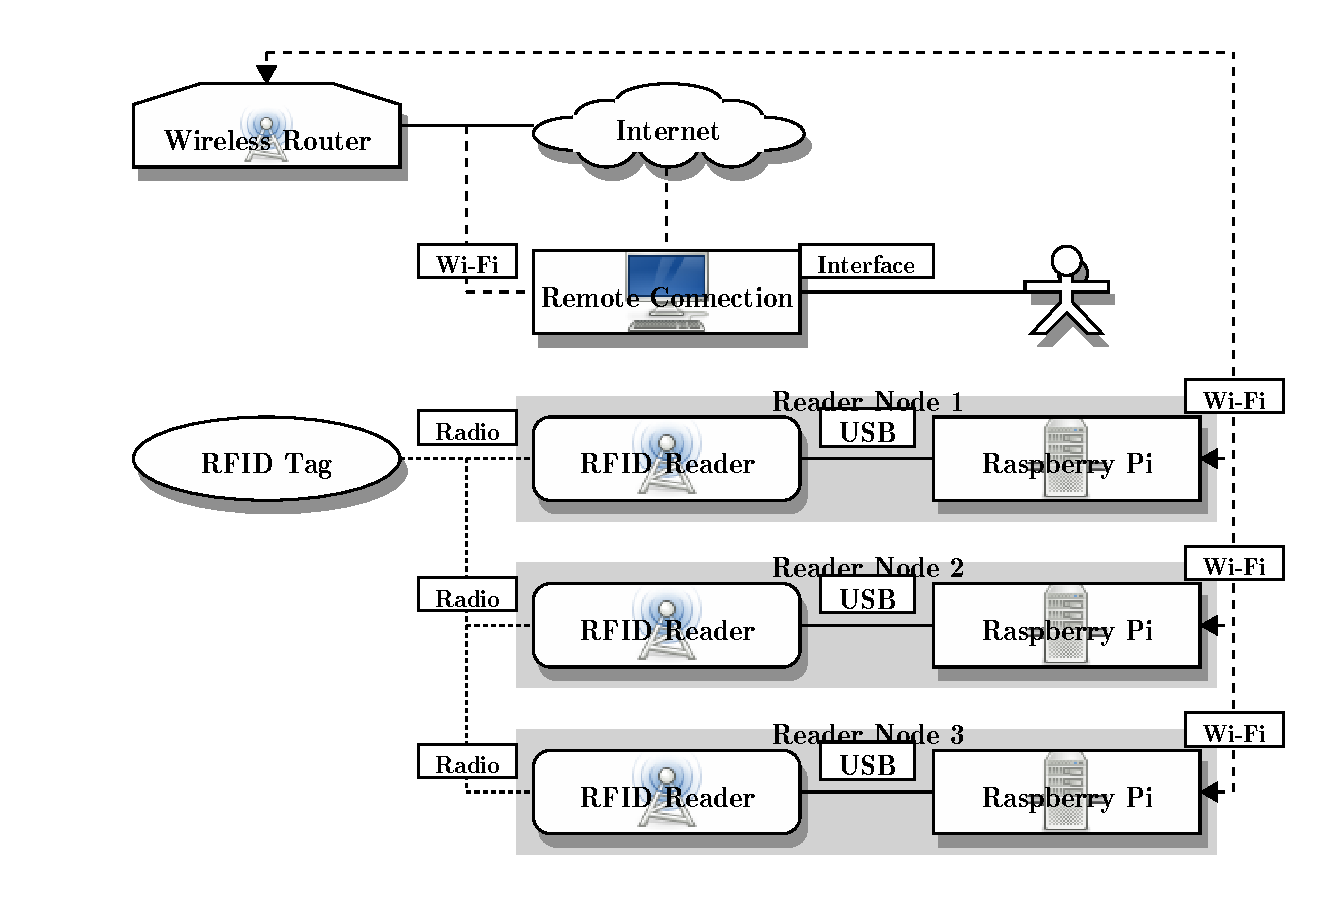
\includegraphics[width=1\textwidth]{figures/blockdiag/hardwaredesignwifi}
		\caption{Hardware setup with wireless connectivity between reader nodes.}
		\label{fig:hardsetwifi}
	\end{center}
\end{figure}

\newpage
\section{Translation tables from RSSI to distance}
\label{sec:trans}

\begin{table}[h]
	\centering
	\begin{tabular}{ | c | c | c || c | c || c | c || c | c || c | c || c | c || c | c | }
		\hline
		Distance 	& 0  & 1  & 1  & 2  & 2  & 3  & 3  & 4  & 4  & 5  & 5  & 6  & 6  & 7  \\ \hline
		RSSI 		& 80 & 65 & 64 & 62 & 61 & 57 & 56 & 53 & 52 & 48 & 47 & 46 & 45 & 44  \\ \hline
	\end{tabular}
	\caption{RSSI value ranges used to estimate distance when using the first reader. }
	\label{tbl:trans1}
\end{table}

\begin{table}[h]
	\centering
	\begin{tabular}{ | c | c | c || c | c || c | c || c | c || c | c || c | c || c | c | }
		\hline
		Distance 	& 0  & 1  & 1  & 2  & 2  & 3  & 3  & 4  & 4  & 5  & 5  & 6  & 6  & 7  \\ \hline
		RSSI 		& 77 & 63 & 62 & 58 & 57 & 55 & 54 &53  & 52 & 49 & 48 & 47 & 46 & 44 \\ \hline
	\end{tabular}
	\caption{RSSI value ranges used to estimate distance when using the second reader. }
	\label{tbl:trans2}
\end{table}

\begin{table}[h]
	\centering
	\begin{tabular}{ | c | c | c || c | c || c | c || c | c || c | c || c | c || c | c | }
		\hline
		Distance 	& 0  & 1  & 1  & 2  & 2  & 3  & 3  & 4  & 4  & 5  & 5  & 6  & 6  & 7  \\ \hline
		RSSI 		& 78 & 64 & 63 & 60 & 59 & 56 & 55 & 54 & 53 & 49 & 48 & 45 & 44 & 43 \\ \hline
	\end{tabular}
	\caption{RSSI value ranges used to estimate distance when using the third reader. }
	\label{tbl:trans3}
\end{table}

\newpage
\section{Orientation of tag to reader}
\label{sec:oriap}

\begin{figure}[H]
	\begin{center}
		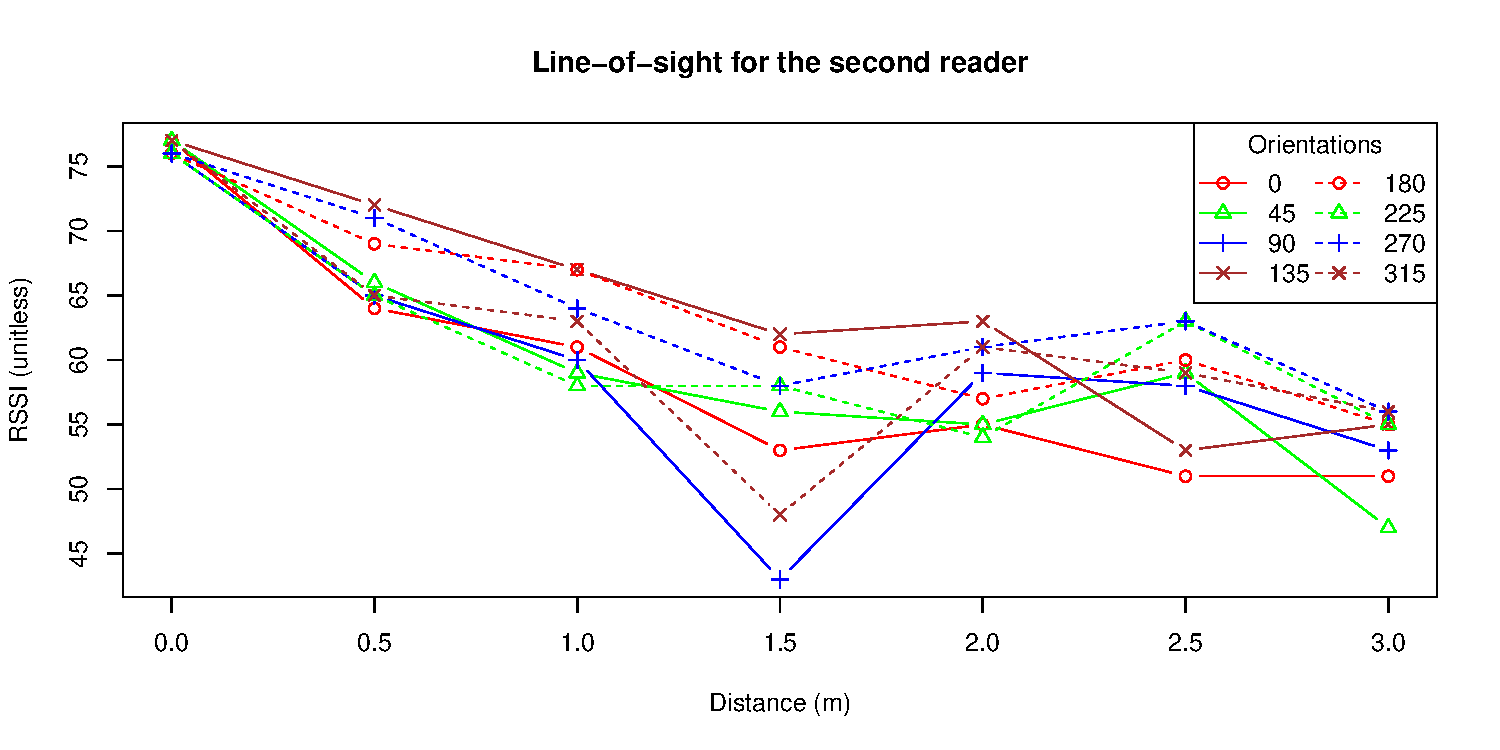
\includegraphics[width=1\textwidth]{figures/rssi_distance_3m_los_r2}
		\caption{Plot of RSSI measurements of different orientations of the tag with respect to the second reader. There was  a line of sight between the RFID devices.}
	\end{center}
\end{figure}

\begin{figure}[H]
	\begin{center}
		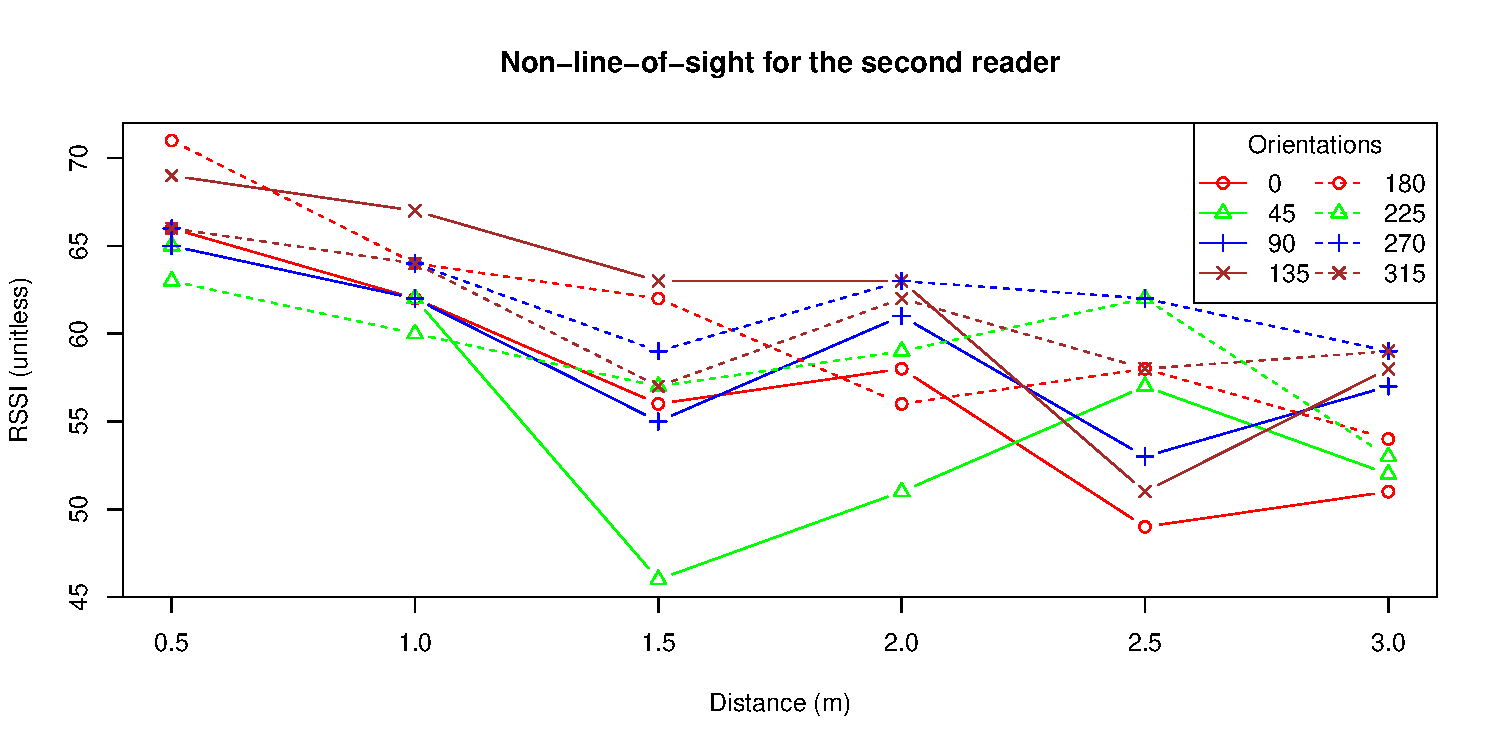
\includegraphics[width=1\textwidth]{figures/rssi_distance_3m_nlos_r2}
		\caption{Plot of RSSI measurements of different orientations of the tag with respect to the second reader. The tag was obscured by an object.}
	\end{center}
\end{figure}

\begin{figure}[H]
	\begin{center}
		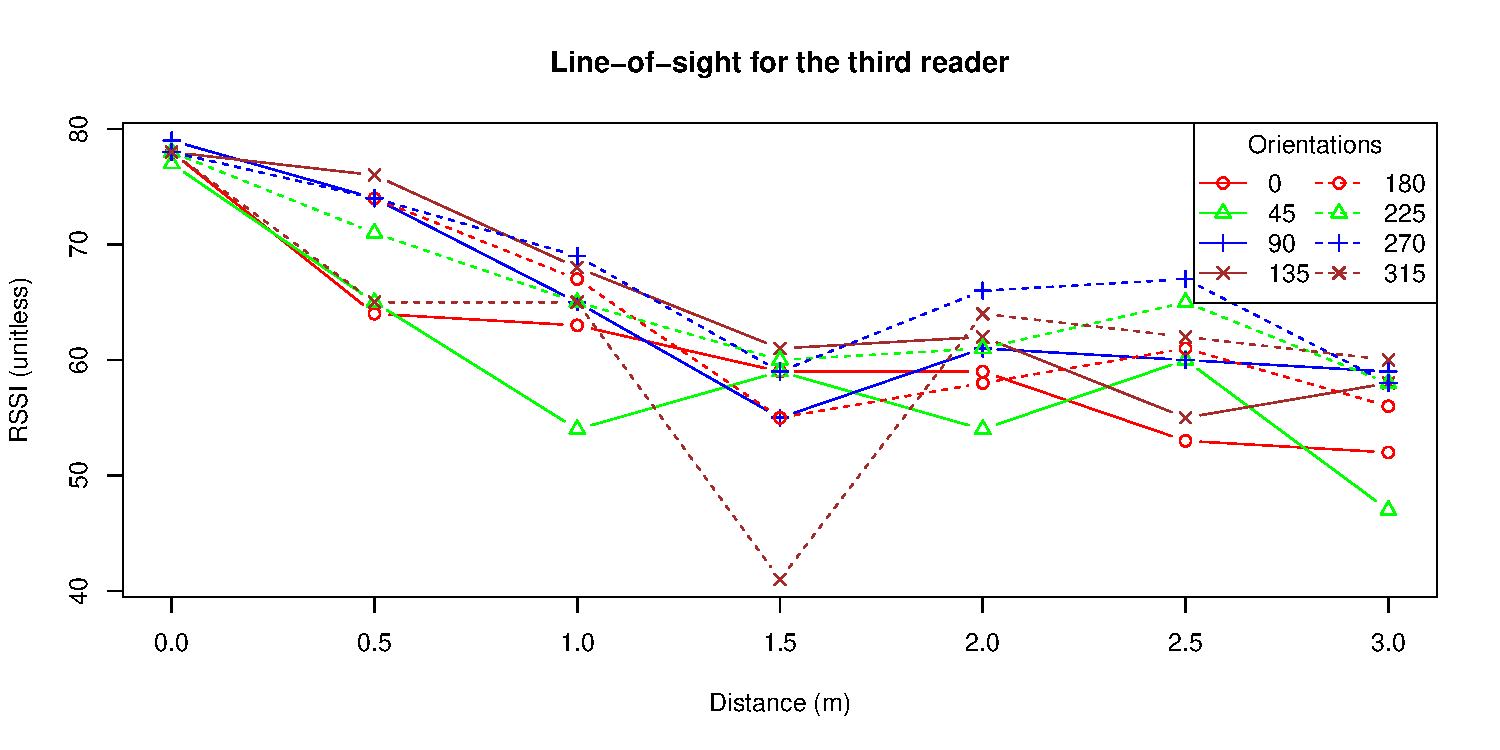
\includegraphics[width=1\textwidth]{figures/rssi_distance_3m_los_r3}
		\caption{Plot of RSSI measurements of different orientations of the tag with respect to the third reader. There was  a line of sight between the RFID devices.}
	\end{center}
\end{figure}

\begin{figure}[H]
	\begin{center}
		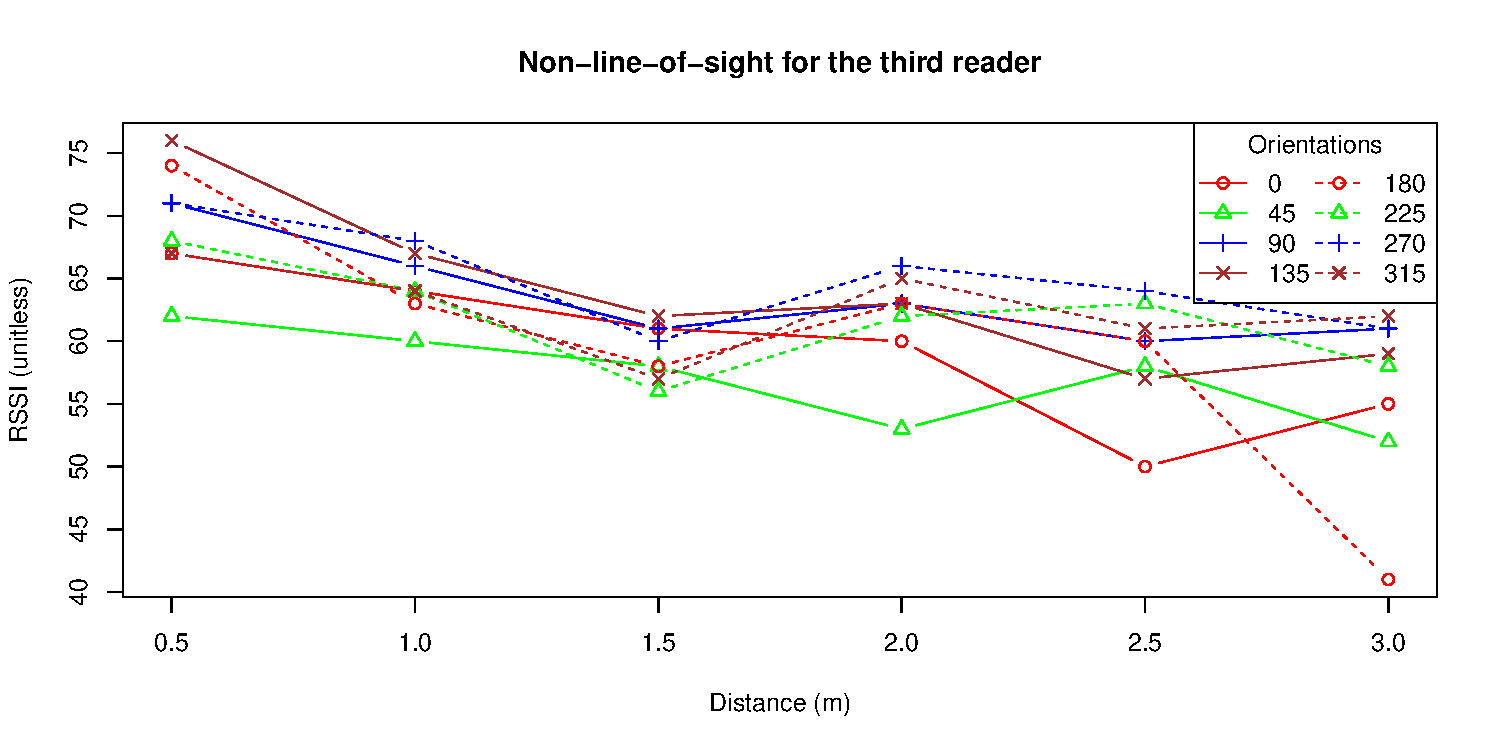
\includegraphics[width=1\textwidth]{figures/rssi_distance_3m_nlos_r3}
		\caption{Plot of RSSI measurements of different orientations of the tag with respect to the third reader. The tag was obscured by an object.}
	\end{center}
\end{figure}

\begin{figure}[H]
	\begin{center}
		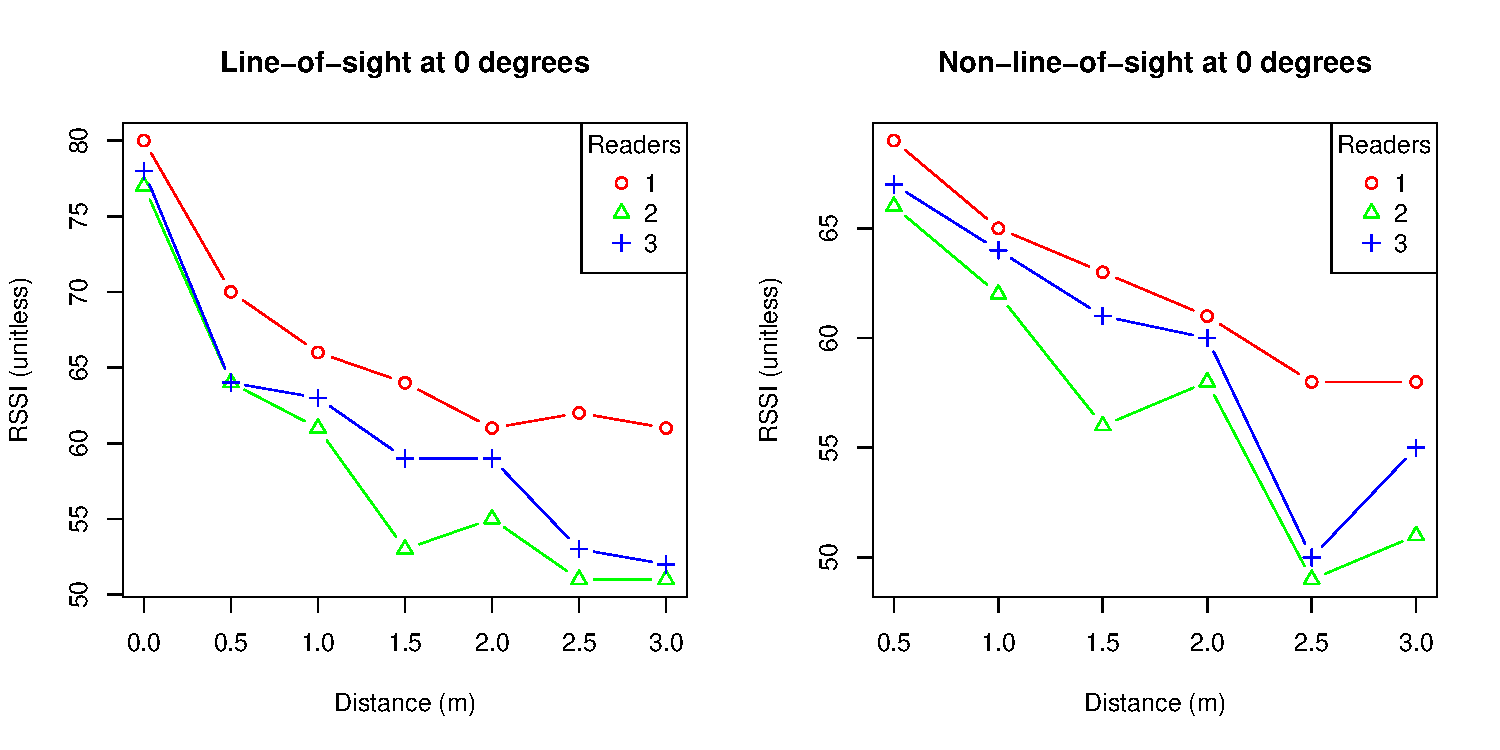
\includegraphics[width=1\textwidth]{figures/rssi_distance_3m_0deg}
		\caption{Two plots of RSSI measurements at increasing distances with the readers at 0 degrees (antennas facing the tag). The left graph show how RSSI values change with a line-of-sight signal propagation. The right graph illustrates the same experiment but with a non-line-of-sight signal propagation (there is an obstacle between the reader and the tag).}
	\end{center}
\end{figure}

\begin{figure}[H]
	\begin{center}
		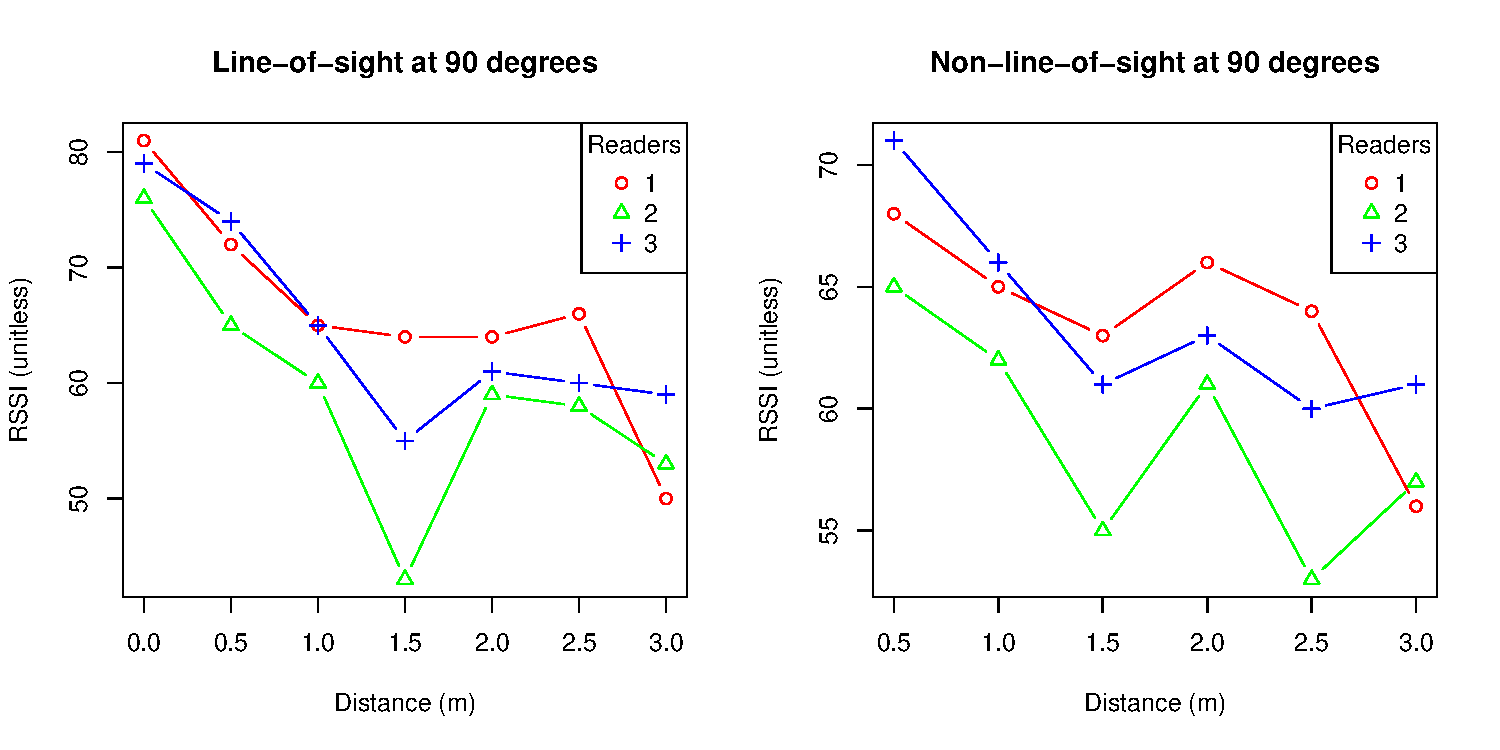
\includegraphics[width=1\textwidth]{figures/rssi_distance_3m_90deg}
		\caption{Two plots of RSSI measurements at increasing distances with the readers at 90 degrees (antennas at an angle to the tag). The left graph show how RSSI values change with a line-of-sight signal propagation. The right graph illustrates the same experiment but with a non-line-of-sight signal propagation (there is an obstacle between the reader and the tag).}
	\end{center}
\end{figure}

\begin{figure}[H]
	\begin{center}
		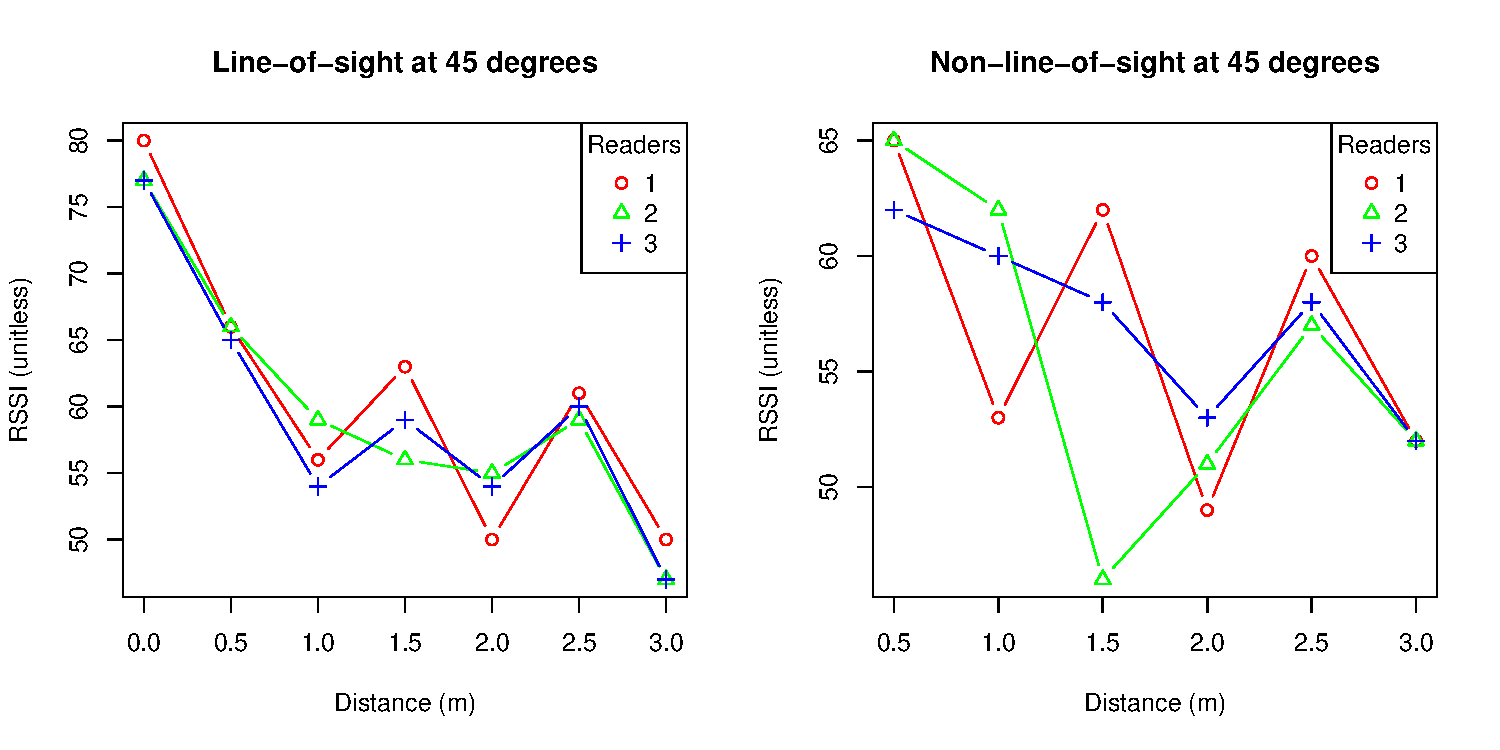
\includegraphics[width=1\textwidth]{figures/rssi_distance_3m_45deg}
		\caption{Two plots of RSSI measurements at increasing distances with the readers at 45 degrees (antennas at an angle to the tag). The left graph show how RSSI values change with a line-of-sight signal propagation. The right graph illustrates the same experiment but with a non-line-of-sight signal propagation (there is an obstacle between the reader and the tag).}
	\end{center}
\end{figure}

\begin{figure}[H]
	\begin{center}
		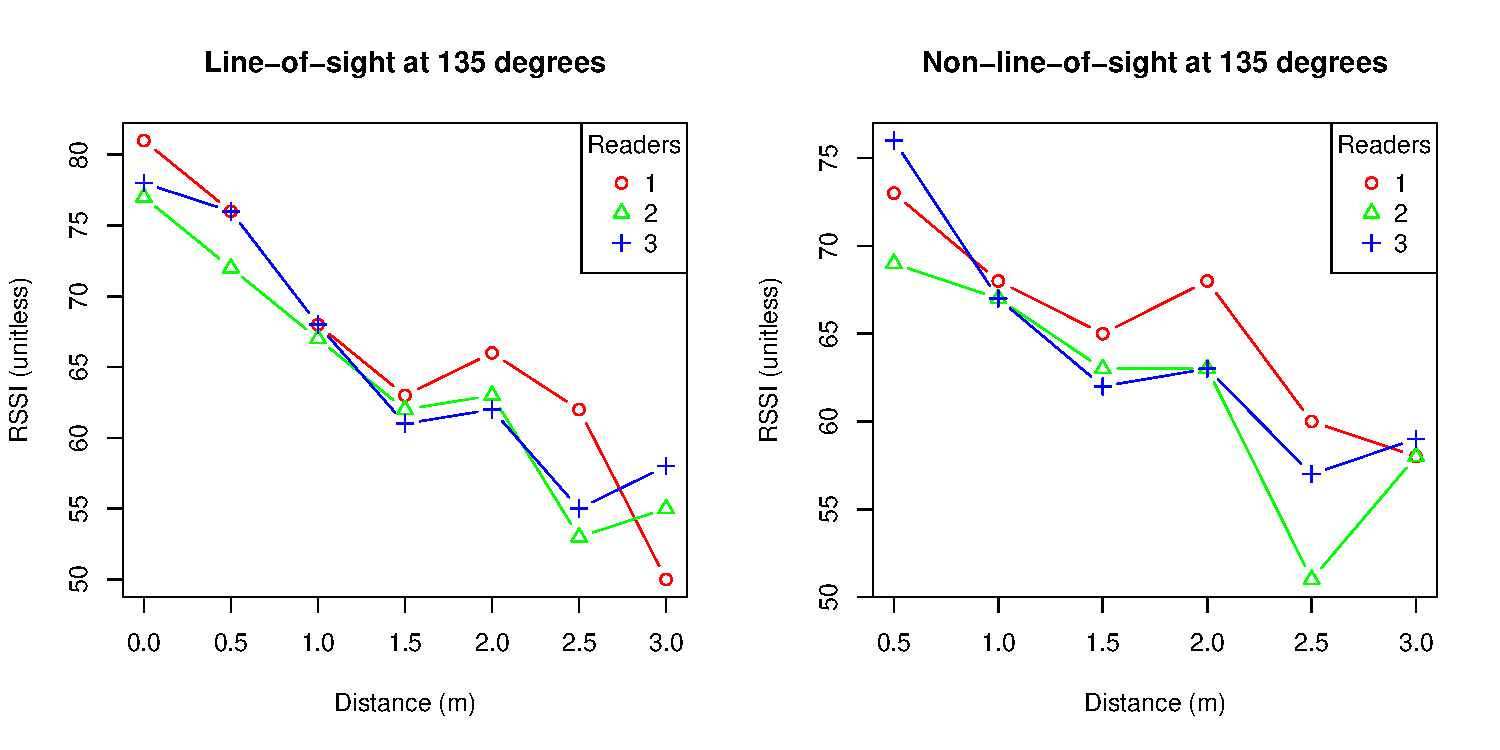
\includegraphics[width=1\textwidth]{figures/rssi_distance_3m_135deg}
		\caption{Two plots of RSSI measurements at increasing distances with the readers at 135 degrees (antennas at an angle to the tag). The left graph show how RSSI values change with a line-of-sight signal propagation. The right graph illustrates the same experiment but with a non-line-of-sight signal propagation (there is an obstacle between the reader and the tag).}
	\end{center}
\end{figure}

\begin{figure}[H]
	\begin{center}
		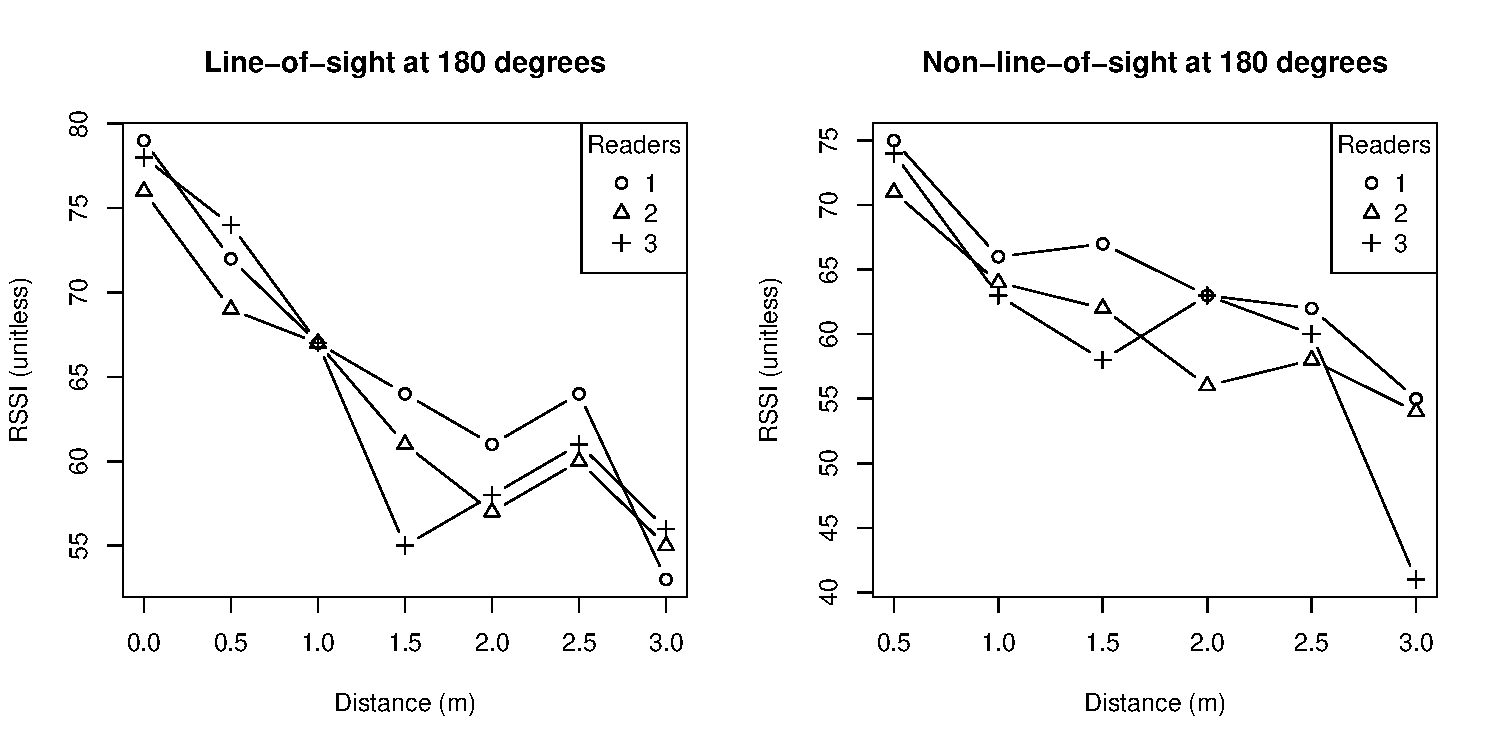
\includegraphics[width=1\textwidth]{figures/rssi_distance_3m_180deg}
		\caption{Two plots of RSSI measurements at increasing distances with the readers at 180 degrees (antennas at an angle to the tag). The left graph show how RSSI values change with a line-of-sight signal propagation. The right graph illustrates the same experiment but with a non-line-of-sight signal propagation (there is an obstacle between the reader and the tag).}
	\end{center}
\end{figure}

\begin{figure}[H]
	\begin{center}
		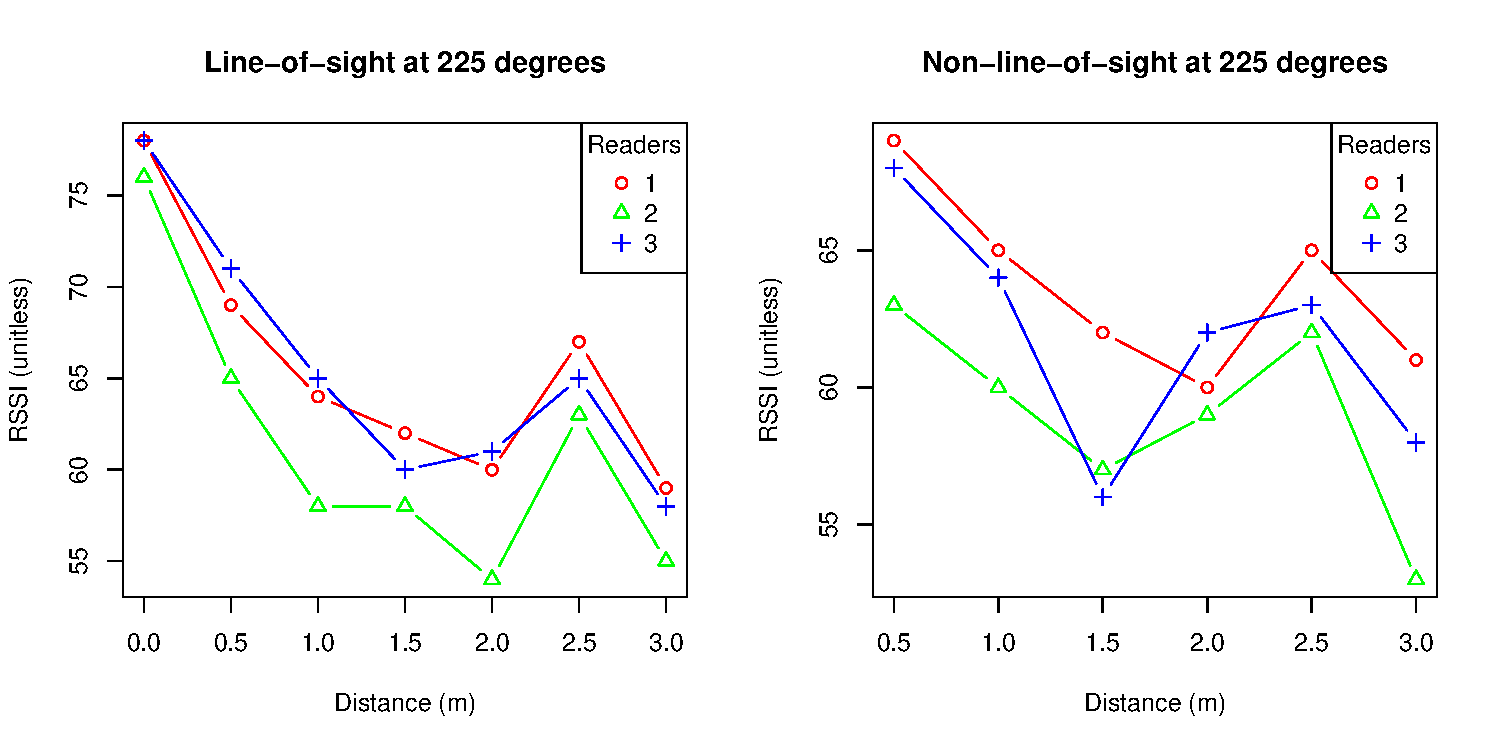
\includegraphics[width=1\textwidth]{figures/rssi_distance_3m_225deg}
		\caption{Two plots of RSSI measurements at increasing distances with the readers at 225 degrees (antennas at an angle to the tag). The left graph show how RSSI values change with a line-of-sight signal propagation. The right graph illustrates the same experiment but with a non-line-of-sight signal propagation (there is an obstacle between the reader and the tag).}
	\end{center}
\end{figure}

\begin{figure}[H]
	\begin{center}
		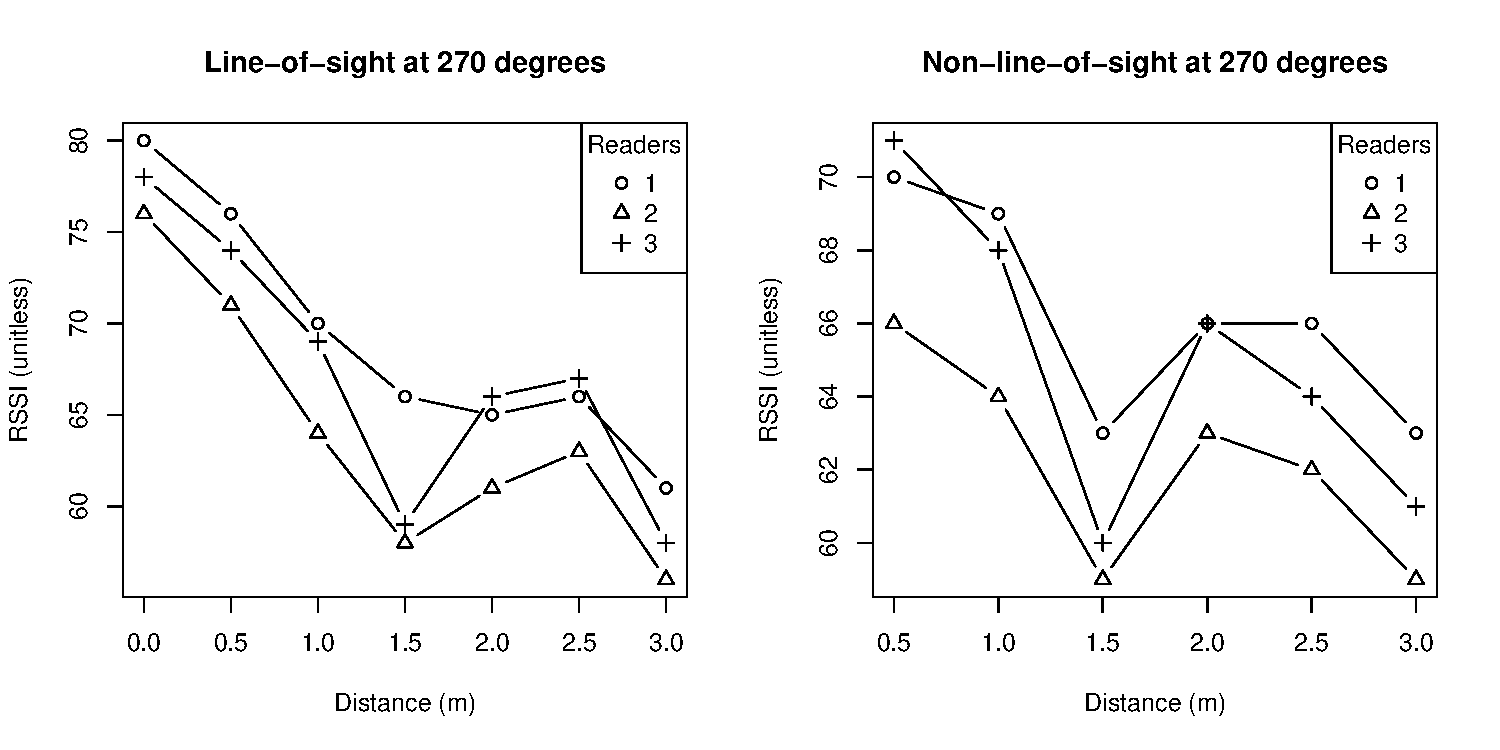
\includegraphics[width=1\textwidth]{figures/rssi_distance_3m_270deg}
		\caption{Two plots of RSSI measurements at increasing distances with the readers at 270 degrees (antennas at an angle to the tag). The left graph show how RSSI values change with a line-of-sight signal propagation. The right graph illustrates the same experiment but with a non-line-of-sight signal propagation (there is an obstacle between the reader and the tag).}
	\end{center}
\end{figure}

\begin{figure}[H]
	\begin{center}
		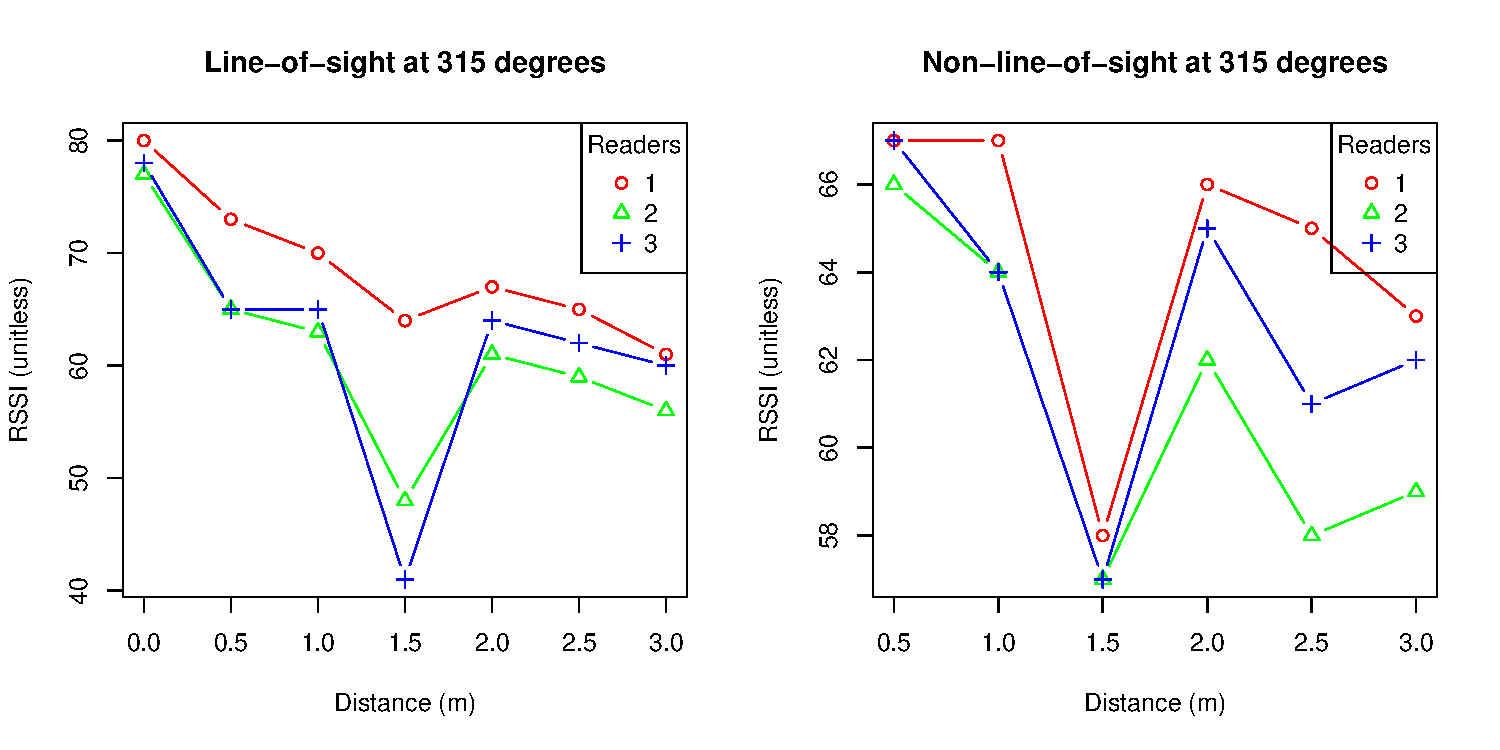
\includegraphics[width=1\textwidth]{figures/rssi_distance_3m_315deg}
		\caption{Two plots of RSSI measurements at increasing distances with the readers at 315 degrees (antennas at an angle to the tag). The left graph show how RSSI values change with a line-of-sight signal propagation. The right graph illustrates the same experiment but with a non-line-of-sight signal propagation (there is an obstacle between the reader and the tag).}
	\end{center}
\end{figure}

\newpage
\section{Grid}

\begin{figure}[H]
	\begin{center}
		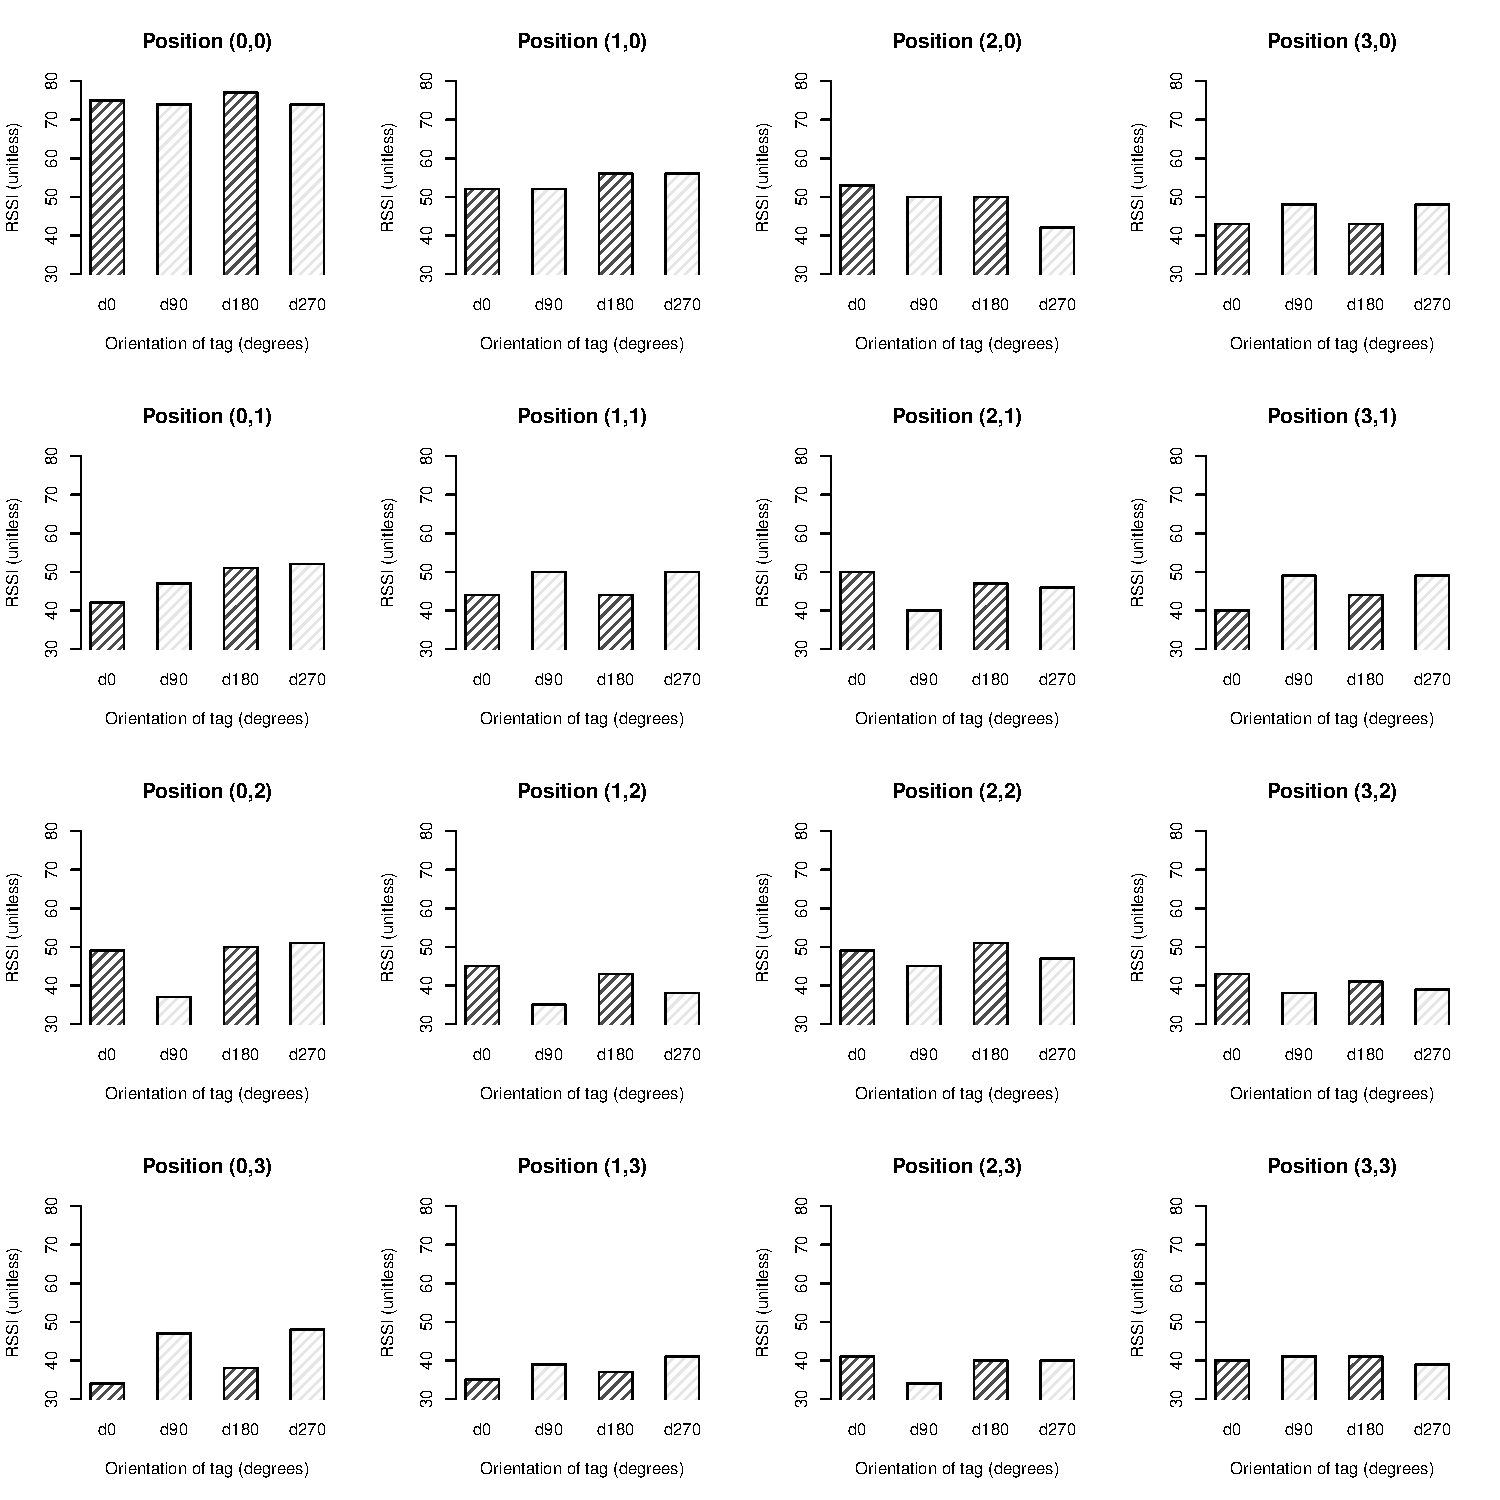
\includegraphics[width=1\textwidth]{figures/rssi_distance_grid_r2}
		\caption{Sixteen plots are organised into a four by four grid. Each plot represents the RSSI measurements of the \textbf{second} reader when the tag is placed at different positions on the x and y axes of the grid. The positions of the tag are all measured in meters. Every four bars in each plot show the RSSI readings when the tag is facing right (0\textdegree), up(90\textdegree), left (180\textdegree), and down (270\textdegree).}
	\end{center}
\end{figure}

\begin{figure}[H]
	\begin{center}
		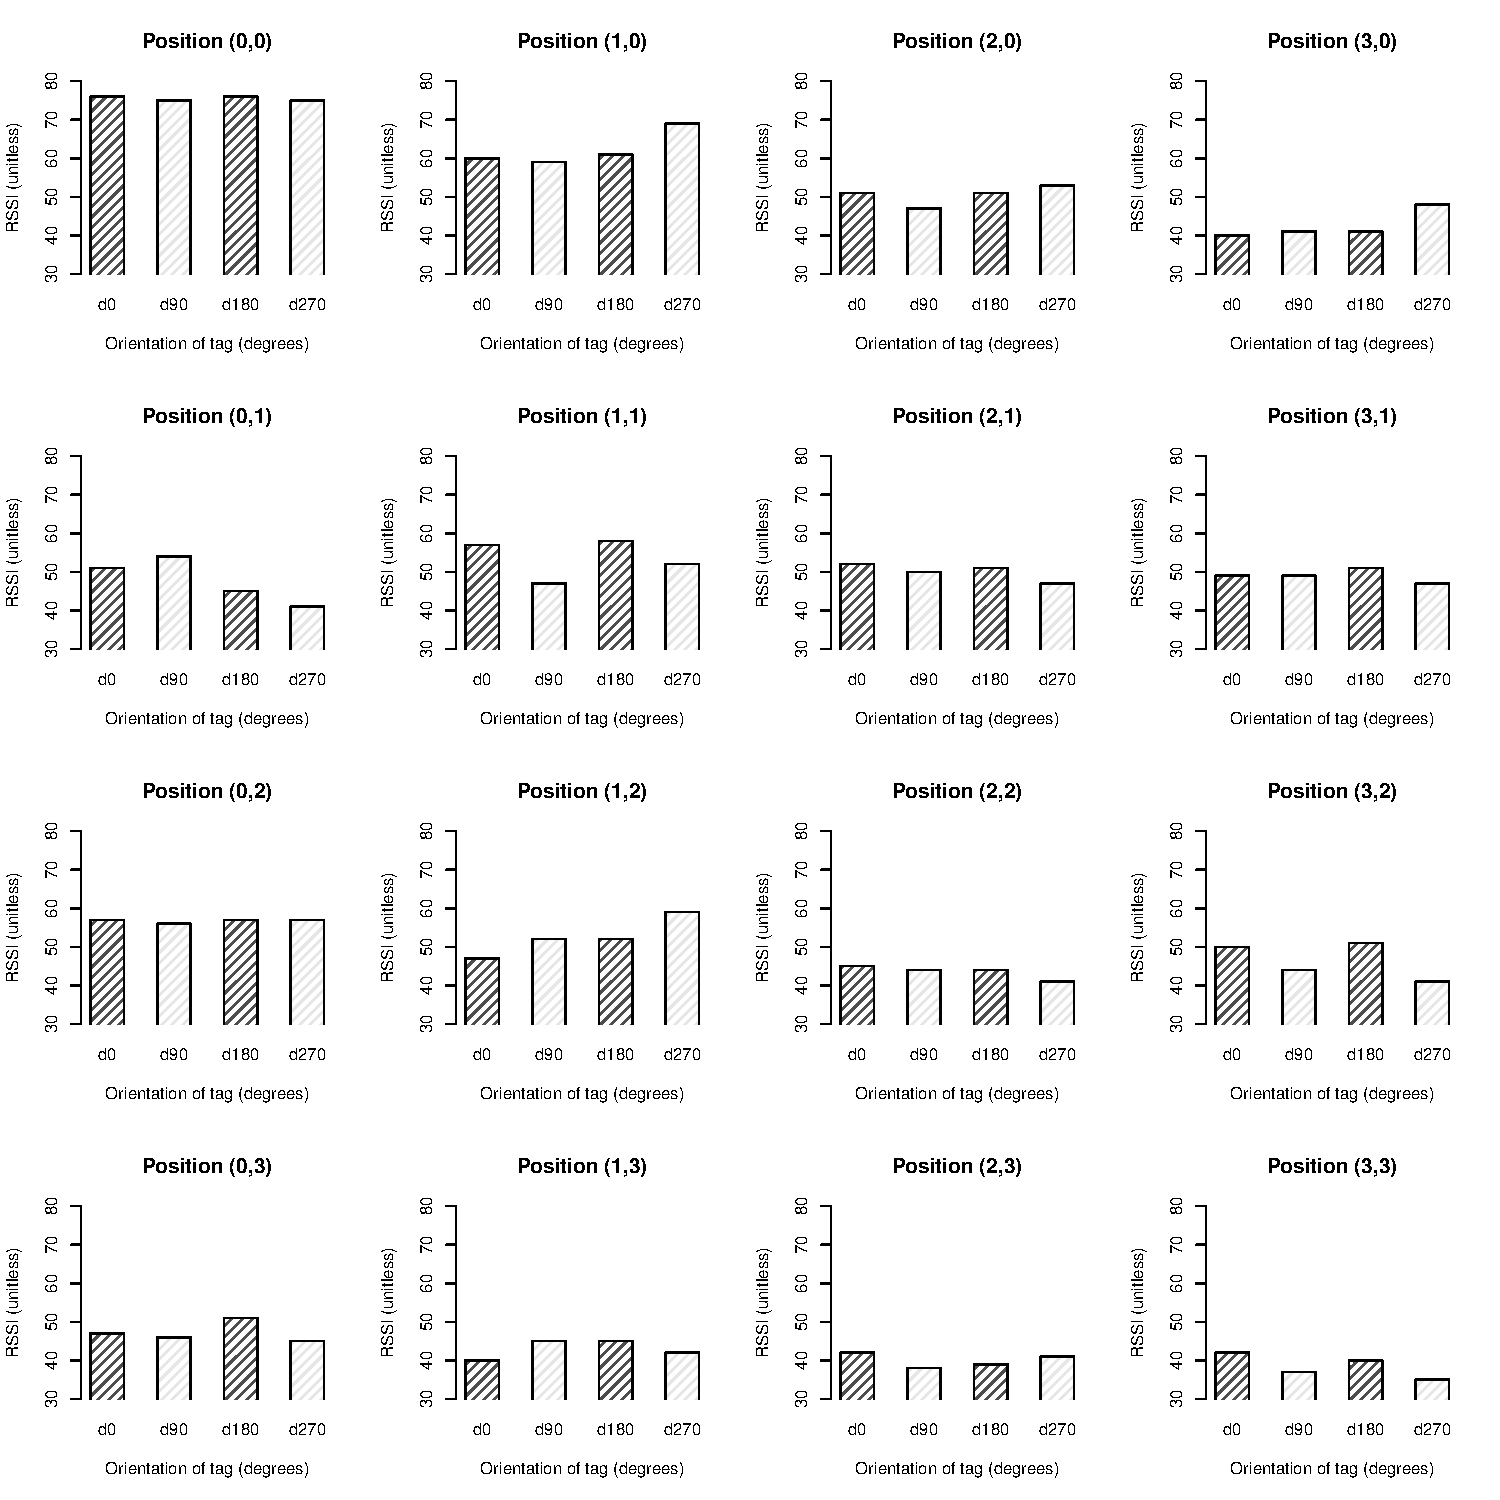
\includegraphics[width=1\textwidth]{figures/rssi_distance_grid_r3}
		\caption{Sixteen plots are organised into a four by four grid. Each plot represents the RSSI measurements of the \textbf{third} reader when the tag is placed at different positions on the x and y axes of the grid. The positions of the tag are all measured in meters. Every four bars in each plot show the RSSI readings when the tag is facing right (0\textdegree), up(90\textdegree), left (180\textdegree), and down (270\textdegree).}
	\end{center}
\end{figure}
